\begin{enumerate}[label=\thechapter.\arabic*,ref=\thechapter.\theenumi]
    \item The Fourier transform X\brak{j\omega} of the signal\\ $x(t)=\frac{t}{\brak{1+t^2}^2}$ is \rule{1.5cm}{0.15mm}.\hfill{GATE-2022-EC-15}
\begin{enumerate}
	\item[(A)] $\frac{\pi}{2j}\omega e^{-\abs{\omega}}$
	\item[(B)] $\frac{\pi}{2}\omega e^{-\abs{\omega}}$
	\item[(C)] $\frac{\pi}{2j}e^{-\abs{\omega}}$
	\item[(D)] $\frac{\pi}{2}e^{-\abs{\omega}}$
\end{enumerate}

\solution
\iffalse
\let\negmedspace\undefined
\let\negthickspace\undefined
\documentclass[journal,12pt,twocolumn]{IEEEtran}
\usepackage{cite}
\usepackage{amsmath,amssymb,amsfonts,amsthm}
\usepackage{algorithmic}
\usepackage{graphicx}
\usepackage{textcomp}
\usepackage{xcolor}
\usepackage{txfonts}
\usepackage{listings}
\usepackage{enumitem}
\usepackage{mathtools}
\usepackage{gensymb}
\usepackage{comment}
\usepackage[breaklinks=true]{hyperref}
\usepackage{tkz-euclide} 
\usepackage{listings}
\usepackage{gvv}                                        
\def\inputGnumericTable{}                                 
\usepackage[latin1]{inputenc}                                
\usepackage{color}                                            
\usepackage{array}                                            
\usepackage{longtable}                                       
\usepackage{calc}                                             
\usepackage{multirow}                                         
\usepackage{hhline}                                           
\usepackage{ifthen}                                           
\usepackage{lscape}
\usepackage[center]{caption} % center the captions to figure

\newtheorem{theorem}{Theorem}[section]
\newtheorem{problem}{Problem}
\newtheorem{proposition}{Proposition}[section]
\newtheorem{lemma}{Lemma}[section]
\newtheorem{corollary}[theorem]{Corollary}
\newtheorem{example}{Example}[section]
\newtheorem{definition}[problem]{Definition}
\newcommand{\BEQA}{\begin{eqnarray}}
\newcommand{\EEQA}{\end{eqnarray}}
\newcommand{\define}{\stackrel{\triangle}{=}}
\theoremstyle{remark}
\newtheorem{rem}{Remark}
\begin{document}

\newcolumntype{M}[1]{>{\centering\arraybackslash}m{#1}}
\newcolumntype{N}{@{}m{0pt}@{}}

\bibliographystyle{IEEEtran}
\vspace{3cm}

\title{GATE 2022 BM 14 Q} 
\author{ee23btech11223 - Soham Prabhakar More% <-this % stops a space
}
\maketitle
\newpage
\bigskip

\renewcommand{\thefigure}{\theenumi}
\renewcommand{\thetable}{\theenumi}

\bibliographystyle{IEEEtran}

\textbf{Question:} $x\brak{t}$ is a real continuous-time signal whose magnitude frequency response
$\abs{X\brak{j\Omega}}$ is shown below. After sampling $x\brak{t}$ at 100 $rad.s^{-1}$, the spectral point P
is down-converted to \rule{1cm}{0.15mm} $rad.s^{-1}$ in the spectrum of the sampled signal.
\hfill{(GATE 2022 BM 14 Q)}
\begin{figure}[h!]
    \renewcommand\thefigure{1}
    \centering
    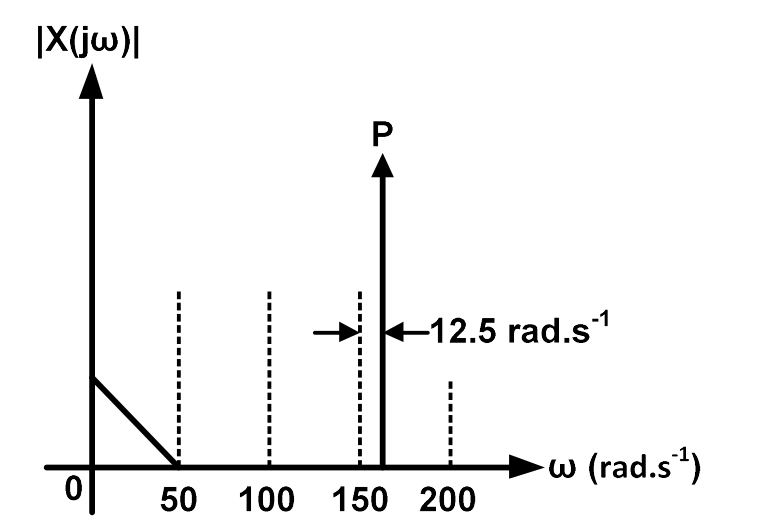
\includegraphics[width=\columnwidth]{2022/BM/14/figs/question.png}
    \caption[short]{Plot of $\abs{X\brak{j\omega}}$}
    \label{fig:2023.bm.14.img1}
\end{figure}

\solution
\fi
\begin{table}[ht]
    \renewcommand\thetable{1}
\begin{tabular}{|c|c|}
    \hline 
    \textbf{Parameter}&\textbf{Description} \\
    \hline
    $w\brak{t}$ & Sampling Function \\
    \hline
	$W\brak{j\omega}$ & Fourier Transform of $w\brak{t}$ \\
    \hline
    $x\brak{t}$ & Input Signal \\
    \hline
    $X\brak{j\omega}$ & Input Signal Frequency Spectrum \\
    \hline
    $x_s\brak{t}$ & Sampled Input Signal \\
    \hline
    $X_s\brak{j\omega}$ & Sampled Signal Frequency Spectrum \\
    \hline
\end{tabular}

\caption{Table of parameters}
\label{Table:1}


\end{table} \\
The sampling function is:
\begin{align}
    w(t) &= \sum_{k = -\infty}^{\infty}\delta\brak{t - \frac{2\pi k}{100}} \\
    W(j\omega) &= 100\sum_{k = -\infty}^{\infty}\delta\brak{j\brak{\omega - 100k}}
\end{align}
then the sampled function: 
\begin{align}
    x_s\brak{t} &= x\brak{t}w\brak{t} \\
    X_s\brak{j\omega} &= X\brak{j\omega} * W\brak{j\omega} \\
    X_s\brak{j\omega} &= \int_{-\infty}^{\infty}X\brak{j\theta}W\brak{j\brak{\omega - \theta}}d\theta \\
    X_s\brak{j\omega} &= 100\sum_{k = -\infty}^{\infty}\int_{-\infty}^{\infty}X\brak{j\theta}\delta\brak{j\brak{\omega - 100k - \theta}}d\theta \\
    X_s\brak{j\omega} &= 100\sum_{k = -\infty}^{\infty}X\brak{j\brak{\omega - 100k}} 
\end{align}
Thus, The down sampled point is at:
\begin{align}
    \omega &= \abs{162.5 - 100k}
\end{align}
where $k$ is the nearest integer to $\frac{162.5}{100}$, which is 2\\
Thus,
\begin{align}
    \omega = 37.5\,rad\,s^{-1}
\end{align}

\begin{figure}[h!]
    \renewcommand\thefigure{2}
    \centering
    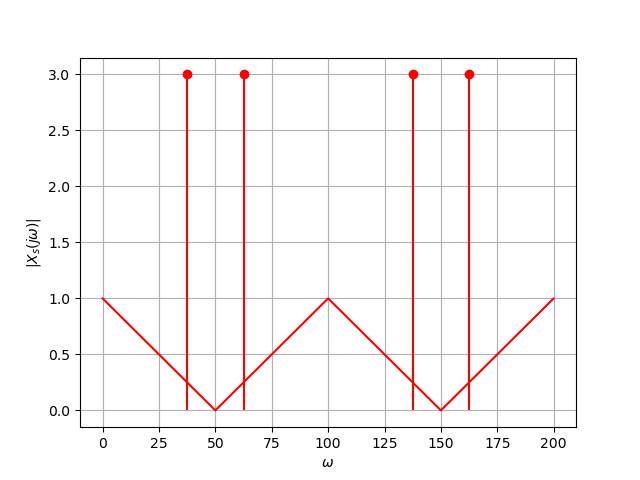
\includegraphics[width=\columnwidth]{2022/BM/14/figs/X_s.png}
    \caption[short]{Plot of $\abs{X_s\brak{j\omega}}$}
    \label{fig:2023.bm.14.img2}
\end{figure}

%\end{document}

\pagebreak

\item For a vector $\bar{x} = [x[0], x[1], \dots, x[7] ]$, the $8$-point discrete Fourier transform (DFT) is denoted by $\bar{X} = \text{DFT}(\bar{x}) = [X[0],X[1],\dots,X[7]]$, where
    \begin{align*}
    X[k] = \sum_{n=0}^{7}x[n]\exp\left(-j\frac{2\pi}{8}nk\right).
    \end{align*} 
    Here $j = \sqrt{-1}$. If $\bar{x} = [1,0,0,0,2,0,0,0]$ and $\bar{y} = \text{DFT}(\text{DFT}(\bar{x}))$, then the value of $y[0]$ is.\hfill{GATE-2022-EC-55}\\
    \solution
    \input{2022/EC/55/55.tex}
    \pagebreak
\item \textbf{Question:} An LTI system is shown in the figure where $$H\brak{s}= \frac{100}{s^2+0.1s+10}$$ The steady state output of the system for an input $x\brak{t}$ is given by $y\brak{t}=a+b\sin{\brak{10t+\theta}}$. The values of $'a'$ and $'b'$ are \\\\
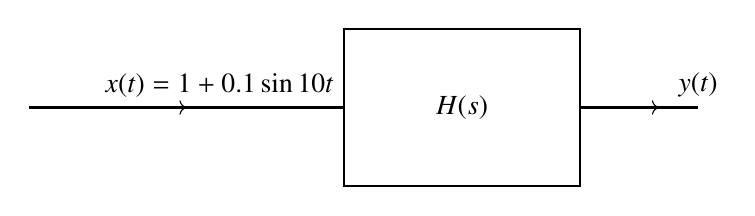
\begin{tikzpicture}
    \draw [thick, draw=black] (-2,-1) -- (2,-1) node[anchor=south east] {$x(t)=1+0.1\sin{\brak{10t}}$};
    \draw [thick,draw=black] (2,0) rectangle (5,-2) ;
    \draw [thick,draw=black] (5,-1) -- (6.5,-1) node[anchor=south] {$y(t)$};
    \draw [->] (-2,-1)--(0,-1);
    \draw [->] (5,-1)--(6,-1);
    \draw (3.5, -1) node[] {$H(s)$};
\end{tikzpicture}\\
\solution 
    \iffalse
\let\negmedspace\undefined
\let\negthickspace\undefined
\documentclass[journal,12pt,twocolumn]{IEEEtran}
\usepackage{cite}
\usepackage{amsmath,amssymb,amsfonts,amsthm}
\usepackage{algorithmic}
\usepackage{graphicx}
\usepackage{textcomp}
\usepackage{xcolor}
\usepackage{txfonts}
\usepackage{listings}
\usepackage{enumitem}
\usepackage{mathtools}
\usepackage{gensymb}
\usepackage{comment}
\usepackage[breaklinks=true]{hyperref}
\usepackage{tkz-euclide} 
\usepackage{listings}
\usepackage{gvv}                                        
\def\inputGnumericTable{}                                 
\usepackage[latin1]{inputenc}                                
\usepackage{color}                                            
\usepackage{array}                                            
\usepackage{longtable}                                       
\usepackage{calc}                                             
\usepackage{multirow}                                         
\usepackage{hhline}                                           
\usepackage{ifthen}                                           
\usepackage{lscape}
\usepackage[center]{caption} % center the captions to figure

\newtheorem{theorem}{Theorem}[section]
\newtheorem{problem}{Problem}
\newtheorem{proposition}{Proposition}[section]
\newtheorem{lemma}{Lemma}[section]
\newtheorem{corollary}[theorem]{Corollary}
\newtheorem{example}{Example}[section]
\newtheorem{definition}[problem]{Definition}
\newcommand{\BEQA}{\begin{eqnarray}}
\newcommand{\EEQA}{\end{eqnarray}}
\newcommand{\define}{\stackrel{\triangle}{=}}
\theoremstyle{remark}
\newtheorem{rem}{Remark}
\begin{document}

\newcolumntype{M}[1]{>{\centering\arraybackslash}m{#1}}
\newcolumntype{N}{@{}m{0pt}@{}}

\bibliographystyle{IEEEtran}
\vspace{3cm}

\title{GATE 2022 BM 14 Q} 
\author{ee23btech11223 - Soham Prabhakar More% <-this % stops a space
}
\maketitle
\newpage
\bigskip

\renewcommand{\thefigure}{\theenumi}
\renewcommand{\thetable}{\theenumi}

\bibliographystyle{IEEEtran}

\textbf{Question:} $x\brak{t}$ is a real continuous-time signal whose magnitude frequency response
$\abs{X\brak{j\Omega}}$ is shown below. After sampling $x\brak{t}$ at 100 $rad.s^{-1}$, the spectral point P
is down-converted to \rule{1cm}{0.15mm} $rad.s^{-1}$ in the spectrum of the sampled signal.
\hfill{(GATE 2022 BM 14 Q)}
\begin{figure}[h!]
    \renewcommand\thefigure{1}
    \centering
    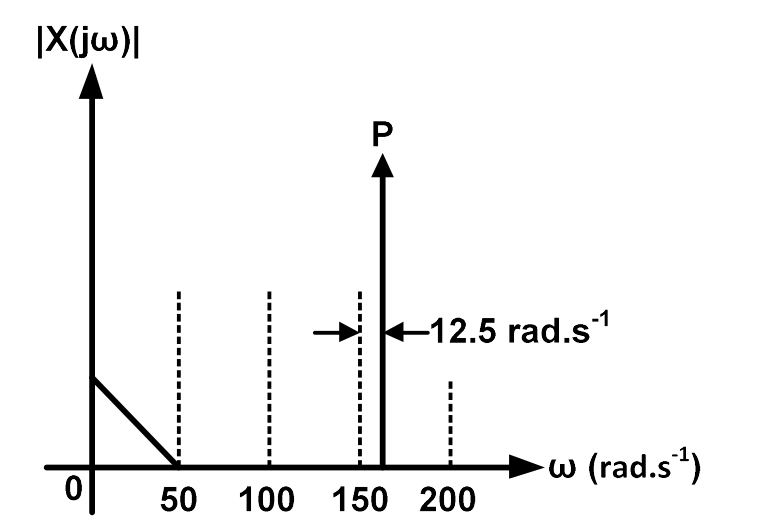
\includegraphics[width=\columnwidth]{2022/BM/14/figs/question.png}
    \caption[short]{Plot of $\abs{X\brak{j\omega}}$}
    \label{fig:2023.bm.14.img1}
\end{figure}

\solution
\fi
\begin{table}[ht]
    \renewcommand\thetable{1}
\begin{tabular}{|c|c|}
    \hline 
    \textbf{Parameter}&\textbf{Description} \\
    \hline
    $w\brak{t}$ & Sampling Function \\
    \hline
	$W\brak{j\omega}$ & Fourier Transform of $w\brak{t}$ \\
    \hline
    $x\brak{t}$ & Input Signal \\
    \hline
    $X\brak{j\omega}$ & Input Signal Frequency Spectrum \\
    \hline
    $x_s\brak{t}$ & Sampled Input Signal \\
    \hline
    $X_s\brak{j\omega}$ & Sampled Signal Frequency Spectrum \\
    \hline
\end{tabular}

\caption{Table of parameters}
\label{Table:1}


\end{table} \\
The sampling function is:
\begin{align}
    w(t) &= \sum_{k = -\infty}^{\infty}\delta\brak{t - \frac{2\pi k}{100}} \\
    W(j\omega) &= 100\sum_{k = -\infty}^{\infty}\delta\brak{j\brak{\omega - 100k}}
\end{align}
then the sampled function: 
\begin{align}
    x_s\brak{t} &= x\brak{t}w\brak{t} \\
    X_s\brak{j\omega} &= X\brak{j\omega} * W\brak{j\omega} \\
    X_s\brak{j\omega} &= \int_{-\infty}^{\infty}X\brak{j\theta}W\brak{j\brak{\omega - \theta}}d\theta \\
    X_s\brak{j\omega} &= 100\sum_{k = -\infty}^{\infty}\int_{-\infty}^{\infty}X\brak{j\theta}\delta\brak{j\brak{\omega - 100k - \theta}}d\theta \\
    X_s\brak{j\omega} &= 100\sum_{k = -\infty}^{\infty}X\brak{j\brak{\omega - 100k}} 
\end{align}
Thus, The down sampled point is at:
\begin{align}
    \omega &= \abs{162.5 - 100k}
\end{align}
where $k$ is the nearest integer to $\frac{162.5}{100}$, which is 2\\
Thus,
\begin{align}
    \omega = 37.5\,rad\,s^{-1}
\end{align}

\begin{figure}[h!]
    \renewcommand\thefigure{2}
    \centering
    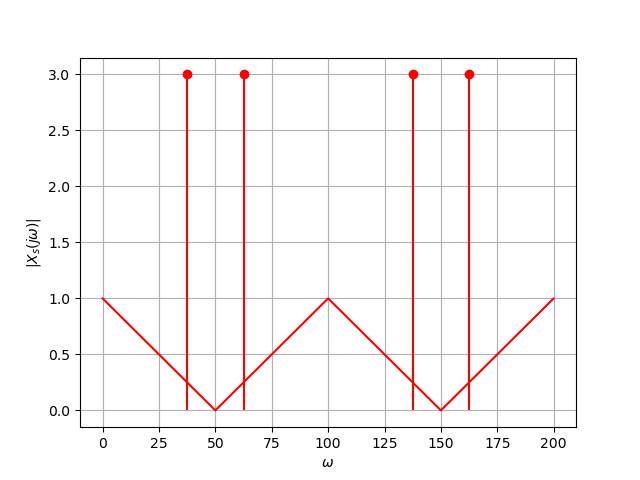
\includegraphics[width=\columnwidth]{2022/BM/14/figs/X_s.png}
    \caption[short]{Plot of $\abs{X_s\brak{j\omega}}$}
    \label{fig:2023.bm.14.img2}
\end{figure}

%\end{document}

\item A periodic function $f(x)$, with period 2, is defined as \\
   \begin{align}   
   f(x) =
   \begin{cases}
    -1-x & -1 \leq x<0 \\
     1-x &  0 <x \leq1 
   \end{cases}
   \end{align} 
   The Fourier series of this function contains \\
\begin{enumerate}[label=\Alph*.]
\item Both $\cos(n\pi x)$ and $sin(n\pi x)$ where n=1,2,3...
\item Only $\sin(n\pi x)$ where n=1,2,3...
\item Only $\cos(n\pi x)$ where n=1,2,3...
\item Only $\cos(2n\pi x)$ where n=1,2,3...  \hfill{GATE IN 2022 }
\end{enumerate} 

\solution
\input{2022/IN/13/g13.tex}
\item  A Simple closed path C in the Complex Plane is shown in the figure.
 \begin{align*}
        \oint_C \frac{2^z}{z^2-1}dz=-\jmath \pi A
 \end{align*}
 Where $\jmath=\sqrt{-1}$, Then find the value of A is \rule{1cm}{0.15mm}(Rounded of to two decimals)
\begin{figure}[h!]
    \centering
    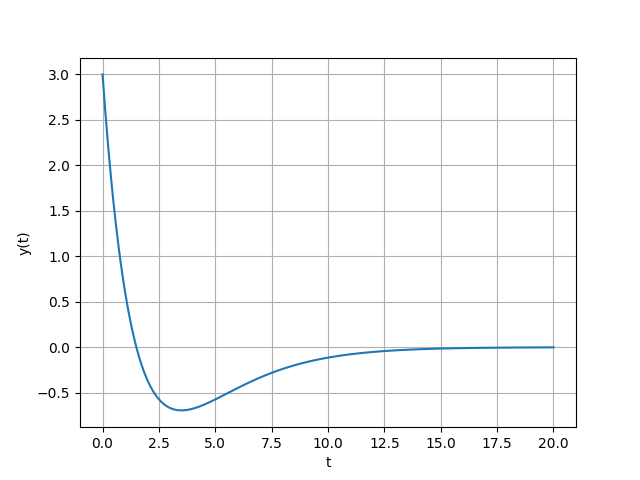
\includegraphics[width = \columnwidth]{2022/EC/32/figs/fig1.png}
\end{figure}
\hfill{(GATE 2022 EC)}\\
\solution 
\input{2022/EC/32/EC_32.tex}
\pagebreak

\item  In the circuit shown below, the switch S is closed at $t=0$. The magnitude of the steady state voltage, in volts, across the $6\Omega$ resistor is \_\_\_\_\_.(\textit{round off to two decimal places})\\ \hfill(GATE 2022 EE Q31)
\begin{figure}[!h]
    \centering
    \begin{circuitikz}[scale = 0.8]
        \draw(0, 0) -- (1, 0);
        \draw(1, 0.5) -- (1, -0.5);
        \draw(4, 0.5) -- (4, -0.5);
        \draw(4, 0) -- (5, 0);

        \draw(1, 0.5) to[R, l = $6\Omega$](4, 0.5);
        \draw(1, -0.5) to[R, l_ = $3\Omega$](4, -0.5);

        \draw(0, 0) -- (0, -2);
        \draw(5, 0) -- (5, -2);

        \draw(0, -2) to[C, l = $1\mu F$](2, -2);
        \draw(2, -2) to [R, l = $10\Omega$](5, -2);

        \draw(0, -2) -- (0, -3.5);
        \draw(5, -2) -- (5, -3.5);

        \draw(0, -3.5) to[battery2, l_ = $10V$](1.5, -3.5);
        \draw (1.5, -3.5) to[switch, l = S] (2, -3.5);
        \draw(2, -3.5) to [R, l = $2\Omega$](5, -3.5);

        \draw[->](0, -3.5) -- (0, -2.5) node[midway, left] {$I$}; 
    \end{circuitikz}
    \caption{}
    \label{fig:1_gate.ee.22.31}
\end{figure}\\
\solution
\iffalse
\let\negmedspace\undefined
\let\negthickspace\undefined
\documentclass[journal,12pt,twocolumn]{IEEEtran}
\usepackage{cite}
\usepackage{amsmath,amssymb,amsfonts,amsthm}
\usepackage{algorithmic}
\usepackage{graphicx}
\usepackage{textcomp}
\usepackage{xcolor}
\usepackage{txfonts}
\usepackage{listings}
\usepackage{enumitem}
\usepackage{mathtools}
\usepackage{gensymb}
\usepackage{comment}
\usepackage[breaklinks=true]{hyperref}
\usepackage{tkz-euclide} 
\usepackage{listings}
\usepackage{gvv}                            \usepackage{tikz}
\usepackage{circuitikz}
\def\inputGnumericTable{}                                
\usepackage[latin1]{inputenc}                            
\usepackage{color}                                       
\usepackage{array}                                       
\usepackage{longtable}                                   
\usepackage{calc}                              
\usepackage{tikz}
\usepackage{multirow}                                    
\usepackage{hhline}                                      
\usepackage{ifthen}                            
\usepackage{caption}
\usepackage{lscape}
\usepackage{amsmath}
\newtheorem{theorem}{Theorem}[section]
\newtheorem{problem}{Problem}
\newtheorem{proposition}{Proposition}[section]
\newtheorem{lemma}{Lemma}[section]
\newtheorem{corollary}[theorem]{Corollary}
\newtheorem{example}{Example}[section]
\newtheorem{definition}[problem]{Definition}
\newcommand{\BEQA}{\begin{eqnarray}}
\newcommand{\EEQA}{\end{eqnarray}}
\newcommand{\define}{\stackrel{\triangle}{=}}
\theoremstyle{remark}
\newtheorem{rem}{Remark}

\begin{document}

\bibliographystyle{IEEEtran}
\vspace{3cm}

\title{GATE 2023 PH Q37}
\author{EE23BTECH11009 - AROSHISH PRADHAN$^{*}$% <-this % stops a space
}
\maketitle
\newpage
\bigskip
\textbf{Question:} In the circuit shown below, the switch S is closed at $t=0$. The magnitude of the steady state voltage, in volts, across the $6\Omega$ resistor is \_\_\_\_\_.(\textit{round off to two decimal places})\\ \hfill(GATE 2022 EE Q31)
\begin{figure}[!h]
    \centering
    \begin{circuitikz}[scale = 0.8]
        \draw(0, 0) -- (1, 0);
        \draw(1, 0.5) -- (1, -0.5);
        \draw(4, 0.5) -- (4, -0.5);
        \draw(4, 0) -- (5, 0);

        \draw(1, 0.5) to[R, l = $6\Omega$](4, 0.5);
        \draw(1, -0.5) to[R, l_ = $3\Omega$](4, -0.5);

        \draw(0, 0) -- (0, -2);
        \draw(5, 0) -- (5, -2);

        \draw(0, -2) to[C, l = $1\mu F$](2, -2);
        \draw(2, -2) to [R, l = $10\Omega$](5, -2);

        \draw(0, -2) -- (0, -3.5);
        \draw(5, -2) -- (5, -3.5);

        \draw(0, -3.5) to[battery2, l_ = $10V$](1.5, -3.5);
        \draw (1.5, -3.5) to[switch, l = S] (2, -3.5);
        \draw(2, -3.5) to [R, l = $2\Omega$](5, -3.5);

        \draw[->](0, -3.5) -- (0, -2.5) node[midway, left] {$I$}; 
    \end{circuitikz}
    \caption{}
    \label{fig:1_gate.ee.22.31}
\end{figure}\\

\solution 
\fi
Consider a sinusoidal input source of angular frequency $\omega$.

\begin{table}[!h]
    \centering
    \begin{tabular}{|c|c|c|}
    \hline
       \textbf{Symbol}  &  \textbf{Value}  &  \textbf{Description}\\
    \hline
       $\omega$  &  $0$ for D.C. &  Angular Frequency\\
    \hline
        $C$ & $1\mu F$ & Capacitance \\
    \hline
        $V_{in}(t)$ & $10\cos(\omega t)$ & Input Voltage\\
    \hline
        $V_{out}(t)$ &  & Output Voltage across $6\Omega$\\
    \hline
        $V_{out}(j\omega)$ & $H(j\omega)V_{in}(j\omega)$ & Output in Frequency Domain\\
    \hline
        $H(j\omega)$ &  & Transfer Function\\
    \hline
        $I(j\omega)$ & & Total Current\\
    \hline
        $Z_{\text{eff}}$ & & Overall Impedance\\
    \hline
    \end{tabular}
    \caption{Given Parameters}
    \label{tab:1_gate.22.ee.31}
\end{table}

Using KCL and KVL, we can calculate:
\begin{align}
    Z_{\text{eff}} &= \frac{2\brak{10 + \frac{1}{j\omega C}}}{12 + \frac{1}{j\omega C}} + 2\\
    \implies I(j\omega) &= \frac{V_{in}}{\brak{\frac{2\brak{10 + \frac{1}{j\omega C}}}{12 + \frac{1}{j \omega C}}+2}}\\
    \implies V_{out}(j\omega) &= 2\sbrak{\brak{\frac{10 + \frac{1}{j\omega C}}{12 + \frac{1}{j\omega C}}}I(j\omega)}\\
    &= 2\sbrak{\brak{\frac{10 + \frac{1}{j\omega C}}{12 + \frac{1}{j\omega C}}}\frac{V_{in}(j\omega)}{\brak{\frac{2\brak{10 + \frac{1}{j\omega C}}}{12 + \frac{1}{j \omega C}}+2}}}\\
    \implies H(j\omega) &= \frac{1 + 10j\omega C}{2(1 + 11j\omega C)}
\end{align}
\begin{figure}[!h]
    \centering
    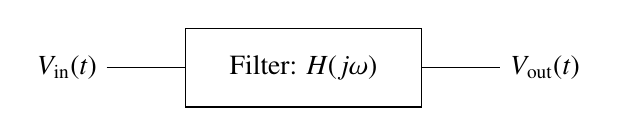
\begin{tikzpicture}
    % Draw the filter rectangle
    \draw (0,0) rectangle (3,1) node[midway] {Filter: $H(j\omega)$};
    
    % Draw the input and output labels
    \draw (-1,0.5) node[left] {$V_{\text{in}}(t)$} -- (0,0.5);
    \draw (3,0.5) -- (4,0.5) node[right] {$V_{\text{out}}(t)$};
\end{tikzpicture}
    \caption{Filter Equivalent of Circuit}
    \label{fig:2_gate.22.ee.31}
\end{figure}
\begin{align}
    H(j\omega) &= \brak{\frac{\sqrt{1 + 100\omega^2 C^2}}{2\sqrt{1 + 121\omega^2 C^2}}}e^{j(\tan^{-1}(10\omega C) - \tan^{-1}(11\omega C))}\\
    &= \brak{\frac{\sqrt{1 + 100\omega^2 C^2}}{2\sqrt{1 + 121\omega^2 C^2}}}e^{j\tan^{-1}\brak{\frac{-\omega C}{1 + 110\omega^2 C^2}}}\\
    \therefore V_{out}(t) &= 10\abs{H(j\omega)}\cos(\omega t + \angle H(j\omega))\\
    &= \frac{5\sqrt{1 + 100\omega^2 C^2}}{\sqrt{1 + 121\omega^2 C^2}}\cos\brak{\omega t -\tan^{-1}\brak{\frac{\omega C}{1 + 110\omega^2 C^2}}}
\end{align}
\begin{figure}[!h]
    \centering
    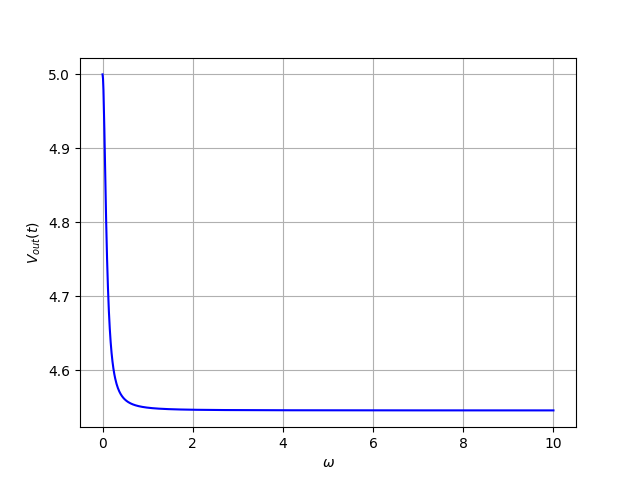
\includegraphics[width = \columnwidth]{2022/EE/31/figs/V_out_plot.png}
    \caption{Plot of $V_{out}(t)$ at $t=0$ w.r.t $\omega$}
    \label{fig:3_gate.22.ee.31}
\end{figure}

As $\omega \rightarrow 0$, $V_{in}(t)$ approaches being a D.C. input source ($10V$).

$\therefore$ substituting $\omega = 0$, we get:
\begin{align}
    V_{out}(t) &= 5V
\end{align}

%\end{document}


\pagebreak
\end{enumerate}
